\section{The Inversion Curse}
\label{sec:cognitive_specialization}

The argument proceeds in four steps. We first evaluate what the unfine-tuned
models can do on the obfuscation tasks, since a post-training reverse
failure is stronger evidence of directional loss when the relevant capability
existed beforehand. We then measure how standard forward fine-tuning affects the
trained direction. We apply BRF to the reverse direction, where the same models
that learn the forward transformation fail to move code back toward the original.
We close with the translation and compilation checks, which reproduce the
directional trend outside the primary testbed.

% \js{shoult'nt we have also had to do a baseline for deobfuscation to compare before and after the finetuning?}\se{paragraph in red below}

\subsection{Baseline Behavior Before Fine-Tuning}
\label{sec:baseline_experiment}

We prompt each unfine-tuned model with a simple zero-shot instruction to
obfuscate the input program under each of the three transformation types:
Identifier Renaming, Dead Code Insertion, and Literal Encryption. We evaluate
the outputs semantically with compilation, execution, and test pass. We evaluate
them syntactically with AST similarity, CodeBLEU, readability, token count, and
cyclomatic complexity.
The open-source models produce executable outputs but apply almost no
transformation. 
%Their AST similarity to the input stays near one. 
Figure~\ref{fig:baseline_comparison}(a) shows low
$AST_{\text{synt}}$ change. Figure~\ref{fig:baseline_comparison}(b) shows
$AST_{\text{struct}}$ near one. Figure~\ref{fig:baseline_comparison}(c)--(d)
show CodeBLEU and readability close to the original program.
Their token counts move by under 5\%. Their CodeBLEU, readability, and cyclomatic complexity
stay close to the original program. 

To check whether this reflects the wording of the task, we also described each transformation explicitly without using the term ``obfuscation''.
We asked the models to rename variables, to insert non-functional code blocks that do not change program behavior, and to replace literals with encrypted forms.
Under these instructions, the open-source models renamed between 23\% and 38\% of unique identifiers, but made no change for dead code insertion or literal encryption.
One possible explanation is that these models rarely saw obfuscation during training and therefore do not recognize it as a task. 
%We do not report these latter results in detail, since our study focuses on obfuscation as a task.
They behave as conservative code generators,
not as obfuscators. This baseline matters for interpretation. A later reverse
failure is unlikely to stem from the model having already mastered a demanding
forward transformation, because the forward transformation is barely present at
baseline.


The GPT models show a different baseline pattern.
Figure~\ref{fig:baseline_comparison}(a) shows moderate lexical change on
Identifier Renaming. They replace roughly 69\% of identifiers
($AST_{\text{synt}}=0.69$), but they produce much less lexical change on Dead Code
Insertion and Literal Encryption, where $AST_{\text{synt}}$ is 0.185 and 0.315.
Figure~\ref{fig:baseline_comparison}(b) shows that structural similarity remains
high across the board, with $AST_{\text{struct}}$ between 0.78 and 0.99. The
baseline changes are mostly lexical rather than structural. About 37\% of GPT
outputs fail because of compilation errors, runtime exceptions, or failed tests.
This suggests that attempts to modify the code introduce semantic alterations
that break executability or test correctness.


A manual review of 100 baseline outputs, split evenly between passing and failing
cases, explains these aggregate scores. Identifier substitutions are generic
names such as \texttt{x} and \texttt{y} rather than deliberate obfuscation.
The code structure stays intact even under prompt-driven obfuscation.
Literal Encryption degrades into dead-code additions rather than genuine
replacement of literal values. The baseline behavior is shallow. The models
imitate the surface form of a transformation without producing the
transformation itself.

The rule-based obfuscator provides a reference point rather than a learning
baseline. It passes tests in 100\% of cases and produces large changes on every
metric. Figure~\ref{fig:baseline_comparison}(c) shows CodeBLEU relative to the
original dropping to 0.50 on Identifier Renaming, 0.33 on Dead Code Insertion,
and 0.22 on Literal Encryption.
These three values are the tool references used later by the
$\mathrm{Acc}_{\text{rev}}$ rule:
$S(C_{\text{tool}},C_{\text{orig}})\in\{0.50,0.33,0.22\}$.
Figure~\ref{fig:baseline_comparison}(d) shows
readability falling from 0.79 to as low as 0.19. Token count rises by 377\%, and
cyclomatic complexity rises by 45\%. Overall,
Figure~\ref{fig:baseline_comparison} shows how far the baseline LLM outputs
remain from that transformation profile.

\begin{figure}[!ht]
    \centering
    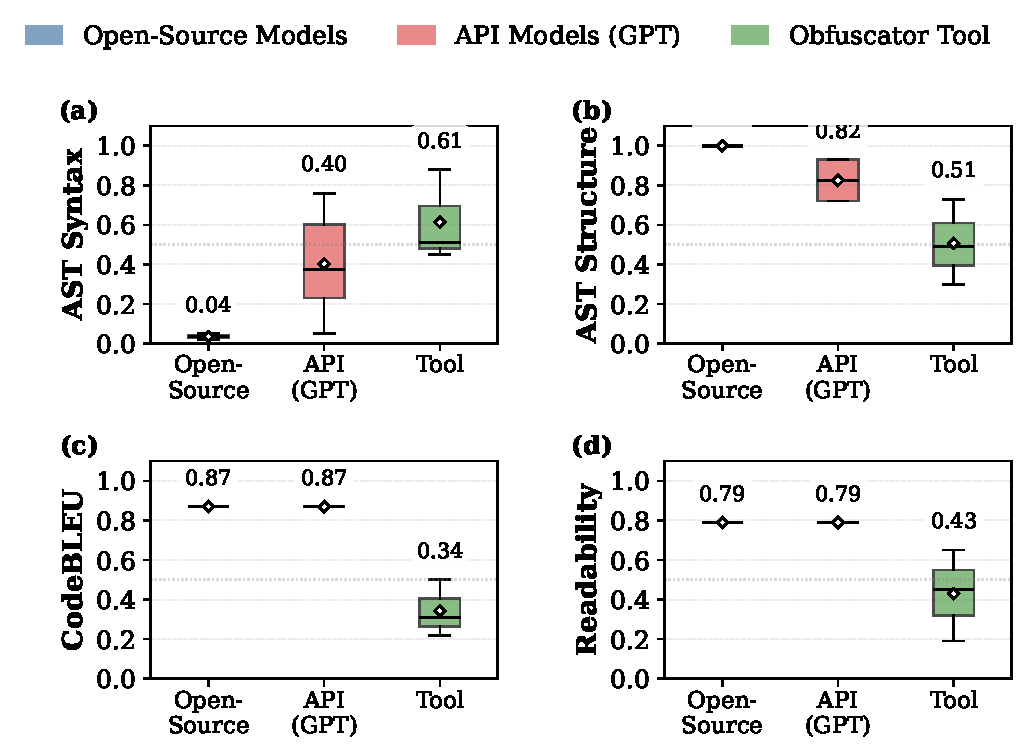
\includegraphics[width=.6\columnwidth, keepaspectratio]{figures/Result_figures/baseline_comparison_boxplot.pdf}
    \caption{Distribution of baseline performance across LLMs.% Open-source
    %models make little measurable change, GPT models make moderate lexical
    %changes, and the rule-based obfuscator produces large divergence from the
    %original program.
    }
    \label{fig:baseline_comparison}
    \vspace{-0.3cm}
\end{figure}




\textbf{Baseline reverse behavior.} We measure the reverse direction before any fine-tuning, so that the
post-fine-tuning reverse results have a point of comparison. 
% The two
The results indicate that they recover a measurable but partial
fraction of the original program on all three transformations.
For GPT-4.1-mini, $\text{Acc}_{\text{rev}}$ is 48.0\% on Identifier Renaming,
49.0\% on Dead Code Insertion, and 32.4\% on Literal Encryption.
GPT-3.5-Turbo reaches 40.2\%, 44.6\%, and 16.8\%.
Dead Code Insertion sits slightly above Identifier Renaming for both API models.
Literal Encryption remains lowest. 
As in the forward baseline, many unsuccessful cases fail at compilation, runtime, or test pass.
The recovery is moderate, not complete. It
registers as movement toward the original on the syntactic metrics
rather than as a return to the original program.
$\mathrm{Acc}_{\text{rev}}$ is decided per program against the tool references
above ($0.50$ / $0.33$ / $0.22$), not by comparing corpus-level means.
For GPT-4.1-mini, mean CodeBLEU of reverse outputs against the original is
$S(C_{\text{deobf}}, C_{\text{orig}}) = 0.440$ on Identifier Renaming,
$0.426$ on Dead Code Insertion, and $0.342$ on Literal Encryption.
Identifier-set overlap moves toward the original, with
$\text{AST}_{\text{synt}}$ gains of $+0.289$, $+0.214$, and $+0.194$.
The outputs sit between the tool-obfuscated input and the original code,
closer to the original but short of full restoration. 

The open-source models, consistent with their near-zero forward transformation at baseline, show negligible reverse recovery before fine-tuning as well. These results suggest that: these models may lack the instruction-following capacity to interpret the reverse prompt without task-specific context or the reverse transformation may exceed their zero-shot reasoning ability; or the scarcity of explicit deobfuscation examples in their pretraining data may make the mapping unrecognizable. Distinguishing these factors is left for future work.


% This reverse baseline uses the two API models, for which the inverse capability is measurable and the fine-tuning interface is controlled. The open-source models apply almost no transformation in either direction at baseline, as the forward results above show, so they provide a weaker reference point for the reverse comparison.






\subsection{Forward Performance After Standard Fine-Tuning}

% We then fine-tune each model on forward pairs and evaluate on the held-out
% ConDefects programs, to confirm that the models learn the forward transformation
% from the supervision they receive. \Cref{fig:model_performance} and
% \Cref{fig:sft_forward_performance} show that standard fine-tuning raises
% forward performance on all three transformations, with gains that vary by task
% type.

We then fine-tune each model with standard fine-tuning (SFT) on forward pairs
only. Each training example maps an original Java program to its
tool-obfuscated counterpart under one transformation type.
The instruction used during fine-tuning is
as follows:

\begin{tcolorbox}[colback=cyan!5, colframe=cyan!25, coltitle=black,
  title=Fine-Tuning Prompt Template, boxrule=0.4pt, left=2pt, right=2pt,
  top=2pt, bottom=2pt]
\small\texttt{Obfuscate the following Java code by \textit{<Obfuscation Technique>}
while preserving its functionality:}\\
\small\textbf{Input: \texttt{<Original code>}} \\
\small\texttt{Here's the obfuscated version preserving functionality:}\\
\small\textbf{Output: \texttt{<Obfuscated code>}}
\end{tcolorbox}

\noindent
Here \texttt{<Obfuscation Technique>} is Identifier Renaming, Dead Code
Insertion, or Literal Encryption. \texttt{<Original code>} is the input and
\texttt{<Obfuscated code>} is the expected tool output. After fine-tuning, we
evaluate on the held-out ConDefects programs with the same instruction format.
\Cref{fig:model_performance} and \Cref{fig:sft_forward_performance} show that
standard fine-tuning raises forward performance on all three transformations,
with gains that vary by task type.

The forward results follow a stable complexity ordering. Identifier Renaming is
learned best, at 68.9\% average success and 81.3\% for GPT-4.1-mini. Dead Code Insertion is harder, at 53.1\% average success and 72.7\% for Mistral. Literal Encryption is hardest, at 20.0\% average success and 29.7\% for Mistral. The ordering holds across models, which indicates that fine-tuning is most effective
when the target transformation reduces to local substitution and least effective
when it requires algorithmic manipulation of program values.

% Auto-correction raises forward results, and its benefit also shrinks with task
% complexity, at 17.6\% on Identifier Renaming, 18.2\% on Dead Code Insertion, and
% 10.1\% on Literal Encryption. The GPT models gain more than the open-source
% models, yet the task ordering is unchanged. An error analysis of the 2{,}805
% failed forward samples explains the pattern. Among them, 63\% compile and run but fail tests, 33\% crash at runtime, and 4\% fail to compile, so the dominant error
% mode is semantic rather than syntactic.


We then apply an iterative auto-correction loop to failed forward outputs.
When a generation fails to compile, execute, or pass tests, we feed the error
message back to the model with a correction prompt. We report results after
five iterations. Further iterations yield no additional gain under our setup.
The correction prompt is as follows:

\begin{tcolorbox}[colback=red!5, colframe=red!25, coltitle=black,
  title=Self-Correction Prompt, boxrule=0.4pt, left=2pt, right=2pt,
  top=2pt, bottom=2pt, fontupper=\small]
\textbf{System:} You are a code obfuscator. The previous obfuscated code did
not work. Here is the code and the error. Please correct the code so it
compiles and passes all tests.\\
\vspace{0.2cm}
\textbf{User:} \\
Original code (for reference):\\
\texttt{<Original Code>}\\
\vspace{0.1cm}
Previous obfuscated code:\\
\texttt{<Generated Code>}\\
\vspace{0.1cm}
Error message:\\
\texttt{<Compiler/Runtime Error or Failed Test Case>}\\
\vspace{0.1cm}
Please correct the code.
\end{tcolorbox}

\noindent
Auto-correction raises forward pass rates. The average gain is 16.6\% on
Identifier Renaming, 19.8\% on Dead Code Insertion, and 13.8\% on Literal
Encryption. GPT-3.5-Turbo rises from 76.3\% to 96.0\% on Identifier Renaming.
GPT-4.1-mini rises from 60.0\% to 88.7\% on Dead Code Insertion.
GPT-3.5-Turbo rises from 22.3\% to 46.7\% on Literal Encryption.
GPT models gain more than the open-source models on average
(20.8 percentage points versus 14.7 across the three transformations).
The gap is concentrated on Dead Code Insertion and Literal Encryption.
\Cref{fig:model_performance} reports the corrected pass rates.

% We measure the link between self-correction gain and transformation
% complexity with Spearman's rank correlation. The association is negative
% ($\rho = -0.85$, $p < 0.01$). 
Average gains stay high on Identifier Renaming
and Dead Code Insertion, where many failures are still recoverable from
compiler or test feedback. Gains shrink on Literal Encryption, where the
failure is usually a wrong program behavior rather than a fixable syntax
fault.
Under our setup, self-correction therefore repairs many surface errors.
It does not close the gap on Literal Encryption. The task
ordering after correction matches the ordering before correction.

We break down the 2{,}705 failed forward samples out of 5{,}400
evaluations.\footnote{Six models, three transformations, 300 evaluation
programs each.} Of these failures, 62\% compile and run but fail tests, 34\% crash at runtime, and
4\% fail to compile. \Cref{fig:errors_xp1} shows the distribution across
models and transformations. The pattern varies by task. On Identifier Renaming,
73\% of failures are incorrect outputs and 21\% are runtime crashes. On Dead
Code Insertion, incorrect outputs remain dominant at 69\%. On Literal
Encryption, runtime crashes rise to 45\% and incorrect outputs fall to 52\%.
Compilation failures stay low on every task (about 3\%--6\% of failures per
transformation). Models often emit code that looks well-formed, while they
still miss the required functional behavior. Appendix reports full details.


\begin{figure}[!ht]
    \centering
    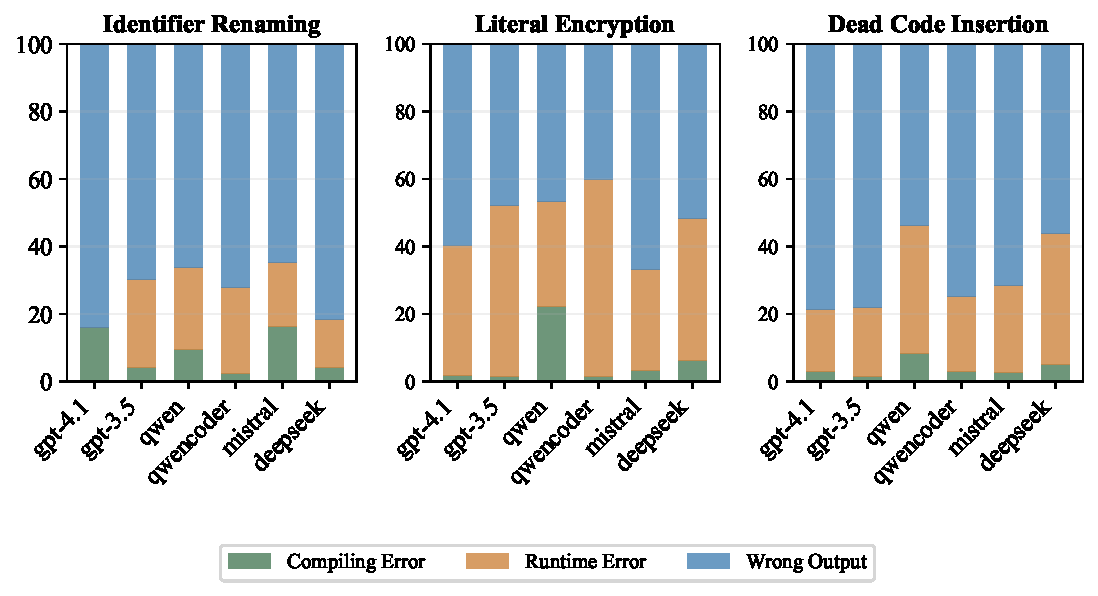
\includegraphics[width=.9\linewidth, height=5cm, keepaspectratio]{figures/figure_reversibility.pdf}
    \caption{Error-type distribution for failed forward outputs after SFT.
    Per-model bars keep the relative error profile of each model and are
    scaled so that each transformation matches the aggregate counts in
    Table~\ref{tab:error_distribution} (2{,}705 failures). Compilation
    failures are rare. Runtime crashes and incorrect outputs that still
    compile account for most failures.}
    \label{fig:errors_xp1}
\end{figure}


%%%%%%%%%%%%%%%%%%%%%%%%%%%%%%

The similarity metrics show that forward fine-tuning shifts model behavior in a
targeted way. On Identifier Renaming, $S(C_{\text{obf}},C_{\text{orig}})$ stays
between 0.42 and 0.50 while $S(C_{\text{obf}},C_{\text{tool}})$ stays between 0.49
and 0.51, a moderate lexical shift toward the tool pattern. On Dead Code
Insertion and Literal Encryption, $S(C_{\text{obf}},C_{\text{orig}})$ falls to
between 0.12 and 0.27 while $S(C_{\text{obf}},C_{\text{tool}})$ rises to between
0.59 and 0.73. Readability follows, from 0.79 on the original code to 0.57 on the
fine-tuned outputs. Standard fine-tuning thus teaches the forward surface pattern
even where full semantic fidelity is not reached.

\begin{figure}[h!]
    \centering
    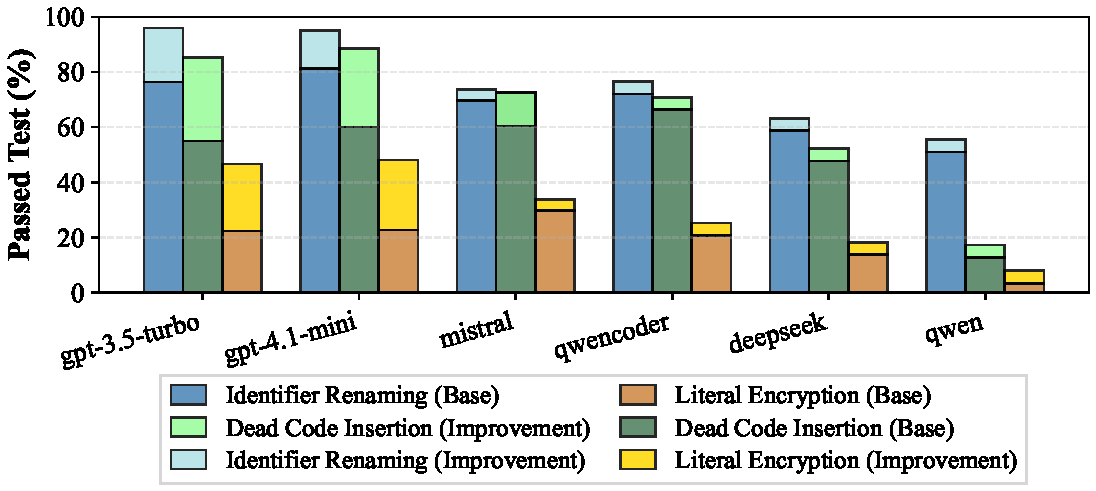
\includegraphics[width=.9\linewidth, height=4cm, keepaspectratio]{figures/model_performance_barplot.pdf}
    \caption{Fine-tuned LLM performance on forward obfuscation.}
    \label{fig:model_performance}
    \vspace{-3mm}
\end{figure}

\begin{figure}[!ht]
    \centering
    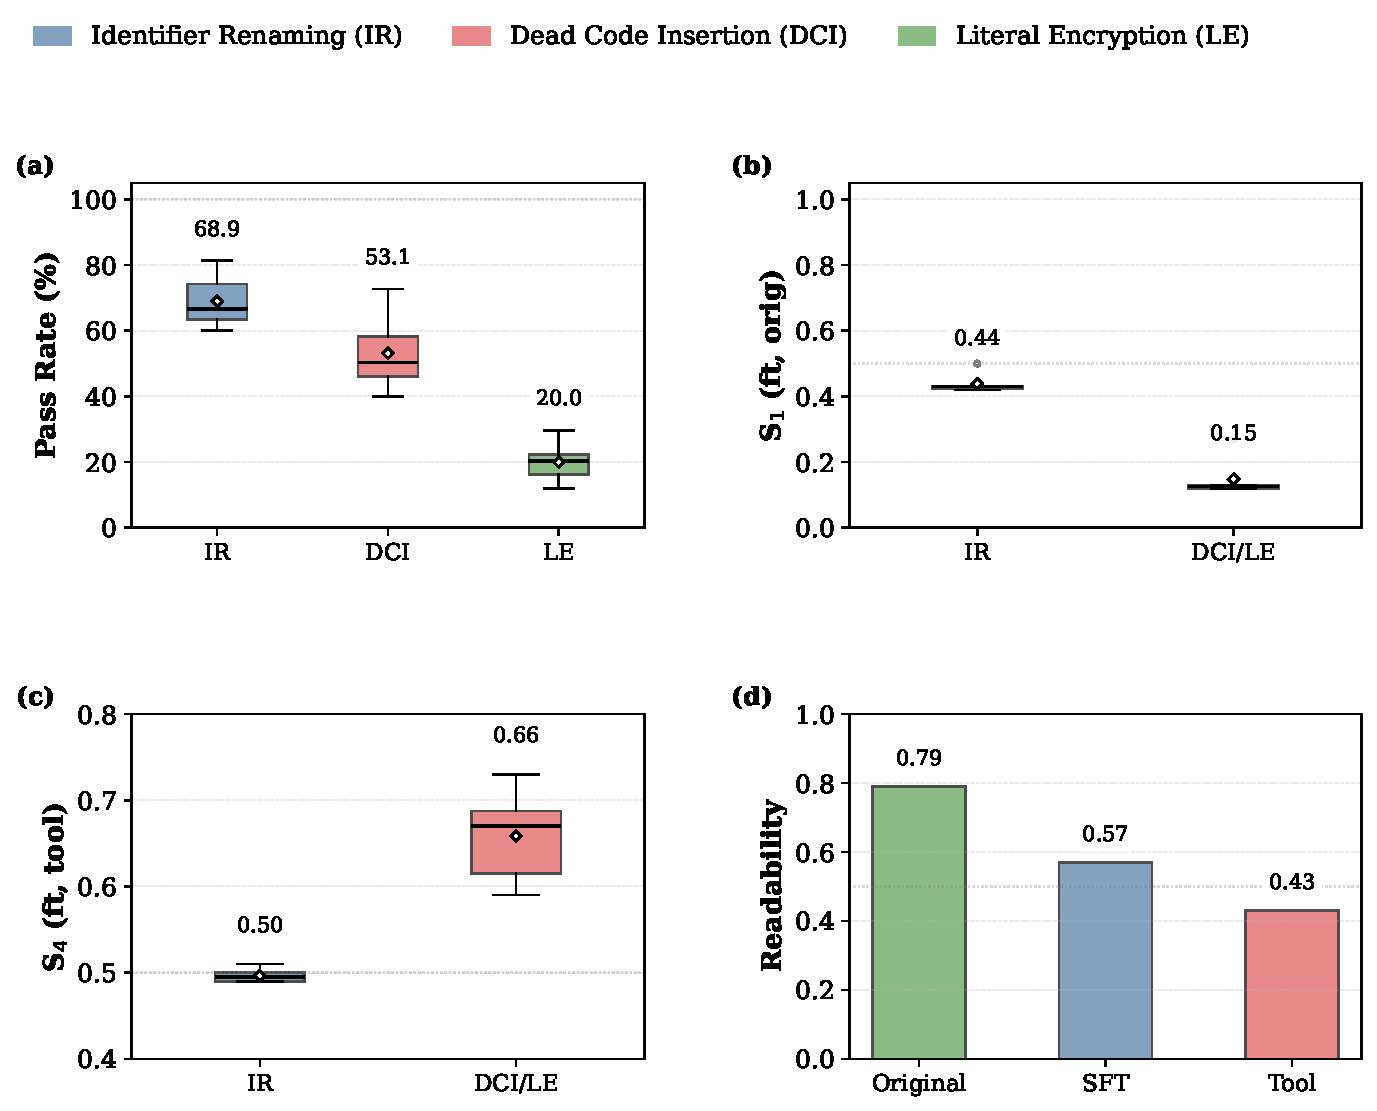
\includegraphics[width=.6\columnwidth, keepaspectratio]{figures/Result_figures/sft_forward_performance.pdf}
    \caption{Forward performance after standard fine-tuning. Pass rates and
    similarity trends show that models learn the forward syntactic pattern more
    reliably than they preserve semantic correctness on the harder tasks.}
    \label{fig:sft_forward_performance}
    \vspace{-0.25cm}
\end{figure}

\subsection{Reverse Evaluation with BRF}
\label{sec:reverse-eval}

%The reverse evaluation is the core result of the paper. 
We prompt every fine-tuned model to deobfuscate tool-generated obfuscated code under four strategies, namely direct instructions, few-shot prompting, chain-of-thought
prompting, and few-shot prompting combined with chain-of-thought. The appendix
lists the full prompts. If forward fine-tuning had preserved any usable inverse
capability, at least one of these strategies would yield outputs that move toward
the original program. None of them does.

Across all six models, all three transformations, and all four prompting
strategies, no output shows net positive movement on any evaluation channel
toward the original program. Reverse recovery is 0\% under the
$\mathrm{Acc}_{\text{rev}}$ rule. Against the reverse
baseline of Section~\ref{sec:baseline_experiment}, the unfine-tuned API
models succeed on 17\% to 49\% of evaluation programs under the same protocol.
This is a drop to zero. %, not a task that was out of reach to begin with. 
 The moderate deobfuscation present before fine-tuning disappears after forward-only
fine-tuning.

This zero is also not an artifact of the word ``deobfuscation''. A model
might fail a reverse prompt because it does not recognize the task label,
even if some inverse capability remained. As in the baseline wording check,
we therefore also prompt the fine-tuned models with reverse instructions that
never use that term. We ask them to restore meaningful identifier names, to
remove non-functional dead-code blocks, and to decrypt AES-encrypted literals
back to their original values. Under these formulations, the models still
emit code that is essentially identical to the obfuscated input. No
evaluation channel moves toward the original program. The result holds even
for Identifier Renaming, where reverse recovery was measurable before
fine-tuning (up to 48.0\% for GPT-4.1-mini). Prompt reformulation does not restore the inverse
mapping. The full prompts appear in the appendix.


%%%%%%%
The zero is not a collapse of generation. The reverse outputs pass the semantic
validity gate. They compile and preserve the behavior of the obfuscated input.
They fail because they do not move toward the original code.
On Identifier Renaming, $AST_{\text{synt}}$ stays near 0.01 against the
obfuscated input, so identifiers barely change.
$AST_{\text{struct}}$ stays at 1.0, so the control-flow skeleton is untouched
(Figure~\ref{fig:cognitive_specialization_fig}(b)).
Token counts move within 3\% of the obfuscated input.
These channels support near-verbatim reproduction of the obfuscated program.
CodeBLEU against the obfuscated input is lower, with
$S(C_{\text{deobf}},C_{\text{tool}})$ between 0.65 and 0.79.
Against the original, mean $S(C_{\text{deobf}},C_{\text{orig}})$ is 0.40 on
Identifier Renaming.
That value stays below the tool reference
$S(C_{\text{tool}},C_{\text{orig}})=0.50$.
On Dead Code Insertion and Literal Encryption, the same comparison uses the
tool references $0.33$ and $0.22$.
Under these references, CodeBLEU does not improve after SFT.
The remaining gap to the obfuscated input is consistent with formatting and
local edits that do not restore the original program.
Figure~\ref{fig:cognitive_specialization_fig}(a) shows the concentration near
the obfuscated endpoint across all three transformations.
Readability does not recover.
On Identifier Renaming, $R(C_{\text{deobf}})$ stays between 0.55 and 0.69,
below the original readability of 0.79.
Dead Code Insertion and Literal Encryption show no readability gain
(Figure~\ref{fig:cognitive_specialization_fig}(c)).

The AST and size metrics confirm that these outputs are near-verbatim
reproductions rather than failed deobfuscations. Across transformation types,
$AST_{\text{synt}}$ stays near 0.01, so identifiers remain almost unchanged,
and $AST_{\text{struct}}$ stays at 1.0, so the control-flow structure is
untouched (Figure~\ref{fig:cognitive_specialization_fig}(b)). Token counts move
within 3\% of the obfuscated input. Readability does not recover. On Identifier
Renaming, $R(C_{\text{deobf}})$ stays between 0.55 and 0.69, below the original
readability of 0.79, and Dead Code Insertion and Literal Encryption show no
readability gain (Figure~\ref{fig:cognitive_specialization_fig}(c)).

Prompting does not change the outcome. Few-shot examples and chain-of-thought
reasoning help when a model holds the underlying capability and needs better task
framing. Here they leave the direction of generation untouched.
Figure~\ref{fig:cognitive_specialization_fig}(d) shows that similarity to the
obfuscated input stays high under Simple, Few-Shot, CoT, and augmented prompts.
The models emit the obfuscated form even when the prompt requests the reverse,
and even when the reasoning trace has begun to describe the reverse mapping
(Figure~\ref{fig:cot_failure_main}). This persistence across prompt forms
separates a prompt mismatch from directional capability loss.

\begin{figure}[!ht]
    \centering
    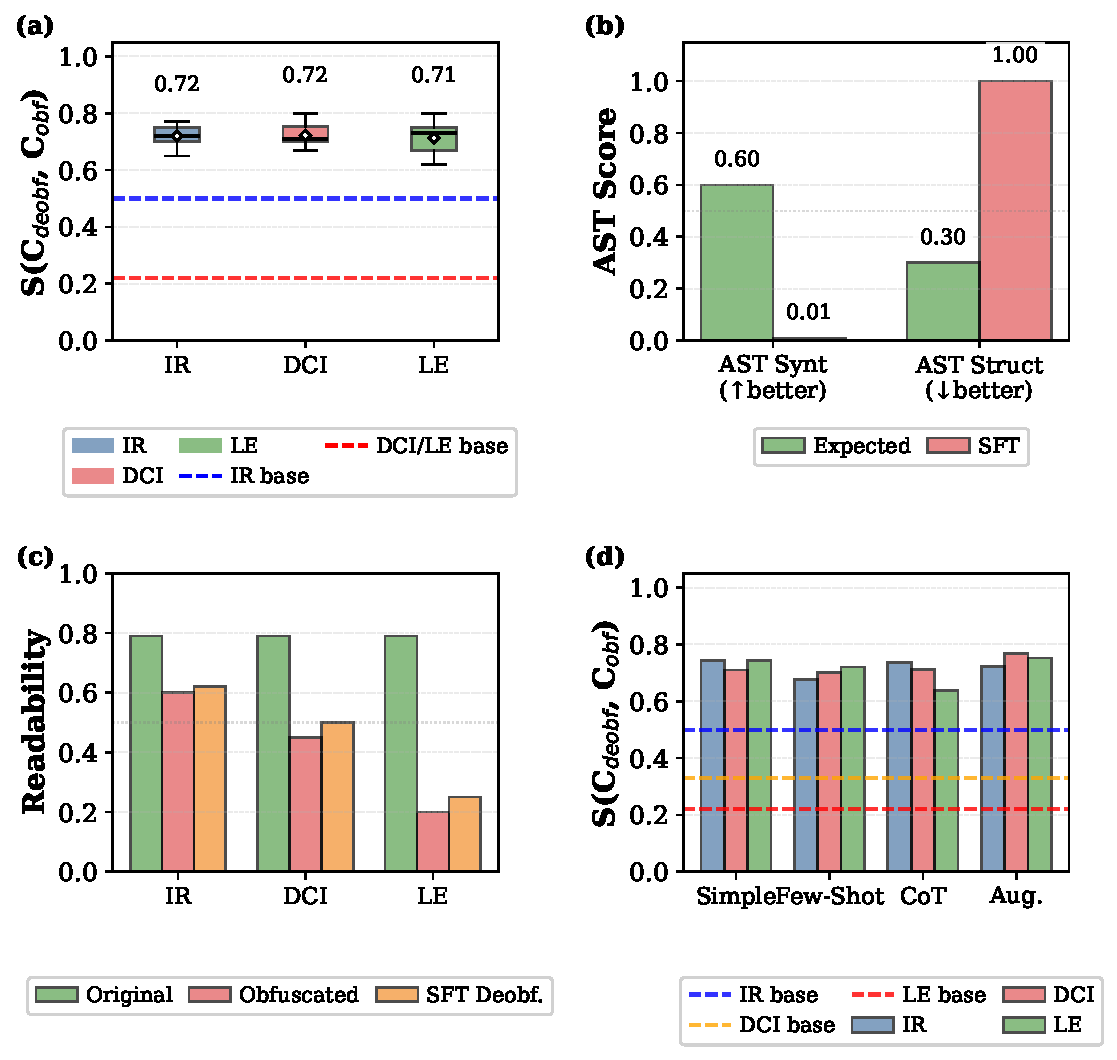
\includegraphics[width=.6\columnwidth, keepaspectratio]{figures/Result_figures/sft_reverse_cognitive_specialization.pdf}
    \caption{Reverse performance after standard fine-tuning. Across models and
    task types, outputs remain concentrated near the obfuscated endpoint instead
    of moving back toward the original program.}
    \label{fig:cognitive_specialization_fig}
\end{figure}

\begin{formal}
Standard fine-tuning creates a large bidirectional gap. The same models that
reach 12.0--81.3\% forward accuracy before self-correction produce 0\%
successful deobfuscation. Identifier, structure, and size metrics show
near-verbatim reproductions of the obfuscated input.
CodeBLEU stays closer to the obfuscated endpoint than to the original, without
reaching full token identity.
This is the defining behavioral signature of the inversion curse.
\end{formal}

\subsection{Directional Loss, Not Global Forgetting}
\label{sec:forgetting-probe}
A large forward-to-reverse gap admits two readings. Adaptation may have
suppressed the specific inverse of the trained transformation, or it may have
degraded the model broadly, in which case unrelated capabilities would fall
alongside the inverse. We separate the two by evaluating the
forward-obfuscation checkpoint, with no further fine-tuning, on its trained
inverse and on two tasks absent from the obfuscation corpus: Python-to-C
translation scored by re-execution, and MBPP code generation. All conditions
use identical prompts, decoding, and scoring.

\begin{table}[t]
\centering
\caption{Directional loss versus global forgetting. Forward-obfuscation
fine-tuning collapses the trained inverse while held-out capabilities stay
near baseline. Values are percentages; $\Delta$ in percentage points.}
\label{tab:forgetting-probe}
\begin{tabular}{@{}lccc@{}}
\toprule
Task & Baseline & Post-FT & $\Delta$ \\
\midrule
Reverse deobfuscation (Java)      & 48.0 & 0.0  & $-48.0$ \\
Python$\rightarrow$C (re-exec.)   & 26.8 & 22.0 & $-4.8$  \\
Code QA (MBPP)                    & 6.0  & 5.7  & $-0.3$  \\
\bottomrule
\end{tabular}
\vspace{-0.5cm}
\end{table}

The inverse collapses while the other tasks do not. Reverse deobfuscation
falls from 48.0\% to 0.0\% ($-48$ pp), whereas Python-to-C moves by $-4.8$ pp
and MBPP by $-0.3$ pp. Global forgetting would pull those two tasks down
together with the inverse. Instead the drop is confined to the direction paired
with the trained transformation. The failure is directional, which is what
separates the inversion curse from catastrophic forgetting and licenses the name.

\subsection{Translation and Compilation Checks}
\label{sec:transl-compil}

The two additional settings reproduce the directional trend under a lighter
protocol. For translation, forward-only fine-tuning on Python-to-Java lowers
Java-to-Python reverse accuracy from a baseline of 85.4\% to 63.3\%. For
compilation, forward-only fine-tuning on C-to-assembly lowers assembly-to-C
reverse accuracy from 16.5\% to 5.5\%. Allowing up to three generations raises translation reverse accuracy to 82.3\% (below the baseline pass@1), while the same allowance barely moves compilation reverse accuracy, at 8.5\%. The pass@3 gap between the two settings distinguishes degraded precision from
directional lock-in: the Java-to-Python capability is weakened but accessible
under repeated sampling, whereas assembly-to-C recovery is blocked regardless
of the number of attempts.

These checks carry less mechanistic detail than the obfuscation study, yet they
establish that the directional pattern is not confined to deobfuscation. The
milder loss under translation and the severe loss under compilation also track
the complexity ordering of the controlled testbed. Reverse performance degrades
less when the inverse approximates a constrained mapping between two high-level
languages, and more when it requires reconstruction from a lower-level
representation.
